\documentclass[a4paper,12pt]{article}
\usepackage[utf8]{inputenc}
\usepackage[T2A]{fontenc}
\usepackage[russian]{babel}
\usepackage{amsmath, amssymb, amsfonts, amsthm}
\usepackage{graphicx}
\usepackage{geometry}
\usepackage{float}
\usepackage[hidelinks, pdfencoding=auto, psdextra]{hyperref}
\usepackage{tocloft}
\usepackage{fancyhdr}
\usepackage{enumitem}
\usepackage{listings}
\usepackage{xcolor}
\usepackage{subcaption}

\geometry{top=2cm, bottom=2cm, left=2cm, right=2cm}
\setlength{\headheight}{14.5pt}

\begin{document}

\begin{titlepage}
    \centering
    {\Large \bfseries Федеральное государственное автономное образовательное учреждение высшего образования «Национальный исследовательский университет ИТМО» \par}
    
    {\large Факультет программной инженерии и компьютерной техники \par}
    \vspace{2cm}
    {\LARGE Домашнее задание №7 \par}
    \vspace{0.5cm}
    \vspace{2cm}
    \vfill
    \begin{flushright}
        \large
        \textbf{Выполнил:} \\
        Шулай Роман \\
        Группа P3115 \\
        \vspace{1cm}
        \textbf{Преподаватель:} \\
        Поляков Владимир Иванович \\
    \end{flushright}
    \vfill
    {\large Санкт-Петербург \\ 2026 год}
\end{titlepage}
\newpage
\setcounter{page}{2}

\textbf{Задача:} \\
Разработать алгоритм, по которому определяется сколько дополнительных серверов нужно поставить, исходя из общей загруженности процессоров и количества запросов на сайт в секунду. \\
Входные данные:
\begin{enumerate}
    \item Общая загруженность процессоров (в процентах от 0 до 100)
    \item Количество запросов на сайт (в RPS - request per second - от 0 до 10000)
\end{enumerate}
Выходные данные: сколько серверов дополнительно нужно поставить (от 0 до 10) \\

\textbf{Шаг 1. Фазификация:} \\
Входная переменная 1: Загруженность процессоров $\{LL, ML, HL\}$
\begin{itemize}
    \item $LL$ (low load) - низкая загруженность
    \item $ML$ (medium load) - средняя загруженность
    \item $HL$ (high load) - высокая загруженность
\end{itemize}
Входная переменная 2: Количество запросов в секунду $\{LRPS, MRPS, HRPS\}$
\begin{itemize}
    \item $LPRS$ (low RPS) - мало запросов в секунду
    \item $MRPS$ (medium RPS) - среднее количество запросов в секунду
    \item $HRPS$ (high RPS) - много запросов в секунду
\end{itemize}
Выходная переменная: Количество дополнительных серверов $\{NS, FS, AS, MS, ES\}$
\begin{itemize}
    \item $NS$ (no servers) - не надо дополнительных установок
    \item $FS$ (few servers) - несколько серверов
    \item $AS$ (average servers) - умеренное количество серверов
    \item $MS$ (many servers) - много серверов
    \item $ES$ (extreme servers) - максимальное количество серверов
\end{itemize}

\textbf{Шаг 2. Блок выработки решения:} \\
Зададим функцию принадлежности для оценки загруженности процессоров $(X)$
\begin{figure}[H]
    \centering
    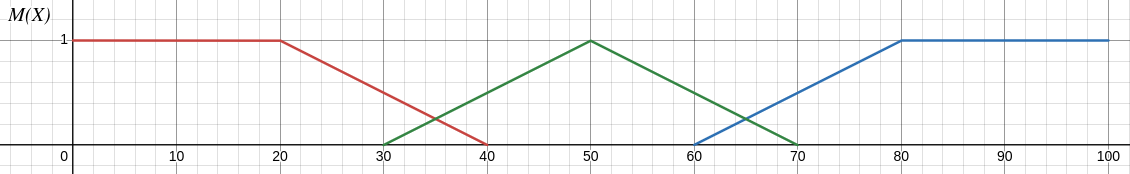
\includegraphics[width=1\linewidth]{images/7/X.png}
\end{figure}

\[
M_{LL}(X) = \begin{cases}
1, & 0 \le X \le 20 \\
-\frac{1}{20}X+2, & 20 \le X \le 40
\end{cases}
\]

\[
M_{ML}(X) = \begin{cases}
\frac{1}{20}X-\frac{3}{2}, & 30 \le X \le 50 \\
-\frac{1}{20}X + \frac{7}{2}, & 50 \le X \le 70
\end{cases}
\]

\[
M_{HL}(X) = \begin{cases}
\frac{1}{20}X-3, & 60 \le X \le 80 \\
1, & 80 \le X \le 100
\end{cases}
\]
\noindent
Зададим функцию принадлежности для оценки количества запросов в секунду $(Y)$
\begin{figure}[H]
    \centering
    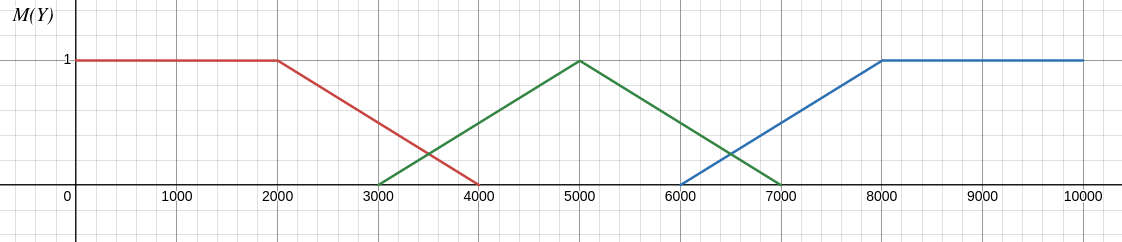
\includegraphics[width=1\linewidth]{images/7/Y.png}
\end{figure}

\[
M_{LRPS}(Y) = \begin{cases}
1, & 0 \le Y \le 2000 \\
-\frac{1}{2000}Y+2, & 2000 \le Y \le 4000
\end{cases}
\]

\[
M_{MRPS}(Y) = \begin{cases}
\frac{1}{2000}Y-\frac{3}{2}, & 30 \le Y \le 50 \\
-\frac{1}{2000}Y + \frac{7}{2}, & 5000 \le Y \le 7000
\end{cases}
\]

\[
M_{HRPS}(Y) = \begin{cases}
\frac{1}{2000}Y-3, & 6000 \le Y \le 8000 \\
1, & 8000 \le Y \le 10000
\end{cases}
\]
\noindent
Зададим функцию принадлежности для оценки количество дополнительных серверов $(Z)$
\begin{figure}[H]
    \centering
    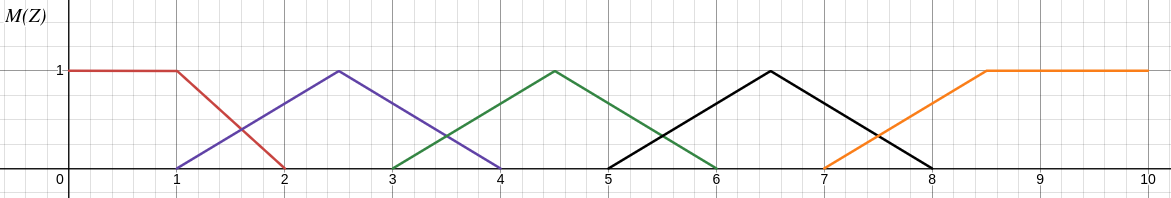
\includegraphics[width=1\linewidth]{images/7/Z.png}
\end{figure}

\[
M_{NS}(Z) = \begin{cases}
1, & 0 \le Z \le 1 \\
-Z + 2, & 1 \le Z \le 2
\end{cases}
\]

\[
M_{FS}(Z) = \begin{cases}
\frac{2}{3}Z-\frac{2}{3}, & 1 \le Z \le 2.5 \\
-\frac{2}{3}Z+\frac{8}{3}, & 2.5 \le Z \le 4
\end{cases}
\]

\[
M_{AS}(Z) = \begin{cases}
\frac{2}{3}Z-2, & 3 \le Z \le 4.5 \\
-\frac{2}{3}Z+4, & 4.5 \le Z \le 6
\end{cases}
\]

\[
M_{MS}(Z) = \begin{cases}
\frac{2}{3}Z-\frac{10}{3}, & 5 \le Z \le 6.5 \\
-\frac{2}{3}Z+\frac{16}{3}, & 6.5 \le Z \le 8
\end{cases}
\]

\[
M_{ES}(Z) = \begin{cases}
\frac{2}{3}Z-\frac{14}{3}, & 7 \le Z \le 8.5 \\
1, & 8.5 \le Z \le 10
\end{cases}
\]
\newpage

\noindent
Создадим базу правил
\begin{table}[H]
    \centering
    \begin{tabular}{|c|c|c|c|}
    \hline
        Загруженность / Запросы & $LRPS$ & $MRPS$ & $HRPS$ \\ \hline
        $LL$ & $NS$ & $NS$ & $FS$ \\ \hline
        $ML$ & $NS$ & $AS$ & $MS$ \\ \hline
        $HL$ & $FS$ & $MS$ & $ES$ \\ \hline
    \end{tabular}
\end{table}

\noindent
Проведем оценку правил. Допустим наши сервера уже загружены на $32\%$, а количество запросов в секунду резко выросло до $RPS=6700$. Определим сколько дополнительных машин нам надо, чтобы выдержать нагрузку.
\begin{enumerate}
    \item Оценим $M_{LL}(X)$ и $M_{ML}(X)$ для $X=32$: 
        \begin{enumerate}
            \item $M_{LL}(X) = -\frac{1}{20}\cdot32+2=0.4$
            \item $M_{ML}(X) = \frac{1}{20}\cdot35-1.5=0.1$
        \end{enumerate}
    \item Оценим $M_{MRPS}(Y)$ и $M_{HRPS}(Y)$ для $Y=6700$:
        \begin{enumerate}
            \item $M_{MRPS}(Y) = -\frac{1}{2000}\cdot6700 + 3.5 = 0.15$
            \item $M_{HRPS}(Y) = \frac{1}{2000}\cdot6700 - 3 = 0.35$
        \end{enumerate}
    \item Выпишем правила которые нужно оценить
        \begin{enumerate}
            \item Низкая загруженность и среднее количество запросов
            \item Средняя загруженность и среднее количество запросов
            \item Низкая загруженность и много запросов
            \item Средняя загруженность и много запросов
        \end{enumerate}
    \item Определим степень истинности для каждого из условий
        \begin{enumerate}
            \item $S_1 = \min(M_{LL}(32),M_{MRPS}(6700))=\min(0.4,0.15)=0.15$
            \item $S_2 = \min(M_{ML}(32),M_{MRPS}(6700)) = \min(0.1,0.15) = 0.1$
            \item $S_3 = \min(M_{LL}(32),M_{HRPS}(6700)) = \min(0.4, 0.35) = 0.35$
            \item $S_4 = \min(M_{ML}(32), M_{HRPS}(6700) = \min(0.1, 0.35) = 0.1$
        \end{enumerate}
    \item $\max(S_1,S_2,S_3,S_4) = S_3 = 0.35$
\end{enumerate}

\textbf{Шаг 3. Дефазификация}\\
Максимальная степень истинности соответствует правилу Few Servers (несколько серверов). Вычислим $Z$, подставив в $M_{FS}$
\begin{gather*}
M_{FS}(Z) = \frac{2}{3}Z-\frac{2}{3} \quad или \quad M_{FS}(Z) = -\frac{2}{3}Z + \frac{8}{3} \\
0.35 = \frac{2}{3}Z-\frac{2}{3} \quad или \quad 0.35 = -\frac{2}{3}Z + \frac{8}{3} \\
Z = 1.525 \quad или \quad Z = 3.475
\end{gather*}
Найдем среднее $Z^* = \frac{1.525+3.475}{2} = 2.5 \approx 3$ \\
Таким образом, оценочное количество дополнительных серверов равно $3$. 


\end{document}